\section{安装Hive}
\subsection{简介}
Hive提供了简化Mapreduce查询的功能,可以输入类SQL语句(HQL或HiveQL)完成对HDFS
中数据的查询。是非常重要的一个工具。

\subsection{配置文件}

\begin{lstlisting}[style=mysh, title=hive-env.sh]
HADOOP_HOME=/opt/hadoop
export HIVE_CONF_DIR=/home/zhangyu/hive/conf	
\end{lstlisting}
\lstinputlisting[style=myxml, title=hive-site.xml]{docs/hive/conf/hive-site.xml}

启动Hive之前,需要配置确保安装和配置好了MySQL,否则会报拒绝连接错误。

\lstinputlisting[style=mysh,title=Hive启动步骤]{docs/scripts/begin_hive.sh}
\subsection{Hive查询与Shell操作}
Hive定义了一套自己的SQL,简称HQL,它与关系型数据库的SQL略有不同,但支持了绝大多数的语句如DDL、DML以及常见的聚合函数、连接查询、条件查询。
DDL操作(数据定义语言)包括:Create、Alter、Show、Drop等。
\begin{enumerate}
\item create database- 创建新数据库
\item alter database - 修改数据库
\item drop database - 删除数据库
\item create table - 创建新表
\item alter table - 变更(改变)数据库表
\item drop table - 删除表
\item create index - 创建索引(搜索键)
\item drop index - 删除索引
\item show table - 查看表
\end{enumerate}

DML操作(数据操作语言)包括:Load 、Insert、Update、Delete、Merge。
\begin{enumerate}
\item load data - 加载数据
\item insert into - 插入数据
\item insert overwrite - 覆盖数据(insert ... values从Hive 0.14开始可用。)
\item update table - 更新表(update在Hive 0.14开始可用,并且只能在支持ACID的表上执行)
\item delete from table where id = 1; - 删除表中ID等于1的数据(delete在Hive 0.14开始可用,并且只能在支持ACID的表上执行)
\item merge - 合并(MERGE在Hive 2.2开始可用,并且只能在支持ACID的表上执行)
\end{enumerate}
注意:频繁的update和delete操作已经违背了Hive的初衷。不到万不得已的情况,还是使用增量添加的方式最好。
\begin{lstlisting}[style=mysh]
$ wget http://192.168.1.100:60000/allfiles/hive3/buyer_log
$ wget http://192.168.1.100:60000/allfiles/hive3/buyer_favorite
$ hive
hive>  create table buyer_log(id string,
buyer_id string,dt string,
ip string,opt_type string)  
 row format delimited fields
  terminated by '\t'  stored as textfile;  
hive> create table buyer_favorite(
	buyer_id string,goods_id string,dt string) 
  row format delimited fields 
  terminated by '\t'  stored as textfile;  
hive> select * from buyer_log limit 10; 
hive> load data local inpath 
'/data/hive3/buyer_log' into table buyer_log;   
hive> load data local inpath 
'/data/hive3/buyer_favorite' into table buyer_favorite; 
hive> select * from buyer_log limit 10;
hive> select l.dt,f.goods_id from buyer_log l,buyer_favorite f 
where l.buyer_id = f.buyer_id limit 10;   
\end{lstlisting}

Hive的语法与SQL类似,不做详细的分析,需要时也能找到很多的资料。下面是将提供的搜狗数据
导入到Hive中的一些脚本。

数据说明如下,其中的分隔符为\lstinline{\t}:

\lstinputlisting[style=mysh,title=sogou-data数据格式说明]{docs/hive/data-desc.txt}

\begin{center}
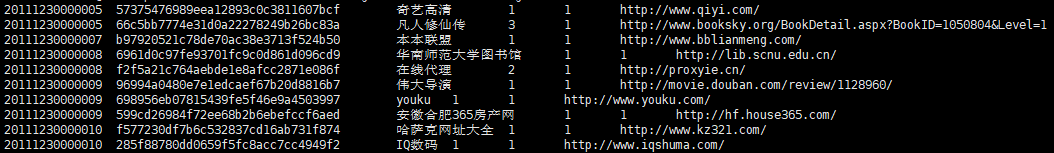
\includegraphics[width=\linewidth]{hive/data-desc.png}
\end{center}

\lstinputlisting[style=mysql,title=sogou-data.sql]{docs/hive/sogou-data.sql}

用Hive来做查询,效率要比编写MR程序再打包提交要高效很多,在实践使用过程
中也能够体会到,Hive查询的时延不是很高,体验较好。

\subsection{Hive JDBC编程}

使用IDEA开发Hive JDBC编程,用Maven管理项目依赖。

启动Hive服务,注意这里使用的不是Cli:
\begin{lstlisting}[style=mysh,title=启动Hive服务]
$ hive --service hiveserver2 &
\end{lstlisting}
\begin{lstlisting}[style=mysh,title=查看Hive服务]
$ netstat -nptl | grep 10000
# 出现监听进程,说明启动正常
\end{lstlisting}
\begin{lstlisting}[style=mysh,title=启动beeline,并尝试连接]
$ beeline
$ !connect jdbc:hive2://master:10000
\end{lstlisting}

在这里连接的时候总是报错,无法连接成功,查看后发现主要是授权的问题,
可是明明用户名和密码都输入正确了。后来通过搜索查看到问题所在,修改Hadoop配置
\lstinline{core-site.xml}文件,添加如下内容取消权限检查,便能够成功进入了。

\begin{lstlisting}[style=myxml]
<property>
      <name>hadoop.proxyuser.zhangyu.hosts</name>
      <value>*</value>
  </property>
  <property>
      <name>hadoop.proxyuser.zhangyu.groups</name>
      <value>*</value>
  </property>
\end{lstlisting}

下面开始新建项目编程:

\begin{lstlisting}[style=myxml,title=POM文件依赖]
<dependency>
  <groupId>org.apache.hive</groupId>
  <artifactId>hive-jdbc</artifactId>
  <version>1.2.1</version>
</dependency>
<dependency>
  <groupId>org.apache.hadoop</groupId>
  <artifactId>hadoop-common</artifactId>
  <version>3.1.2</version>
</dependency>
\end{lstlisting}

注意这里的\lstinline{hive-jdbc}版本用的是1.2.1,而不是Hive的3.1.1。
因为发现使用3.1.1时,有依赖无法解决,一直飘红。所以找了一个使用量比较高的版本1.2.1,因为测试比较简单,仅仅是输出打印,降低版本
后能够正常运行了。

\lstinputlisting[style=customjava,title=HiveDemo.java]{docs/hive/HiveDemo.java}

程序运行截图如下:

\begin{figure}[h]
  \centering
  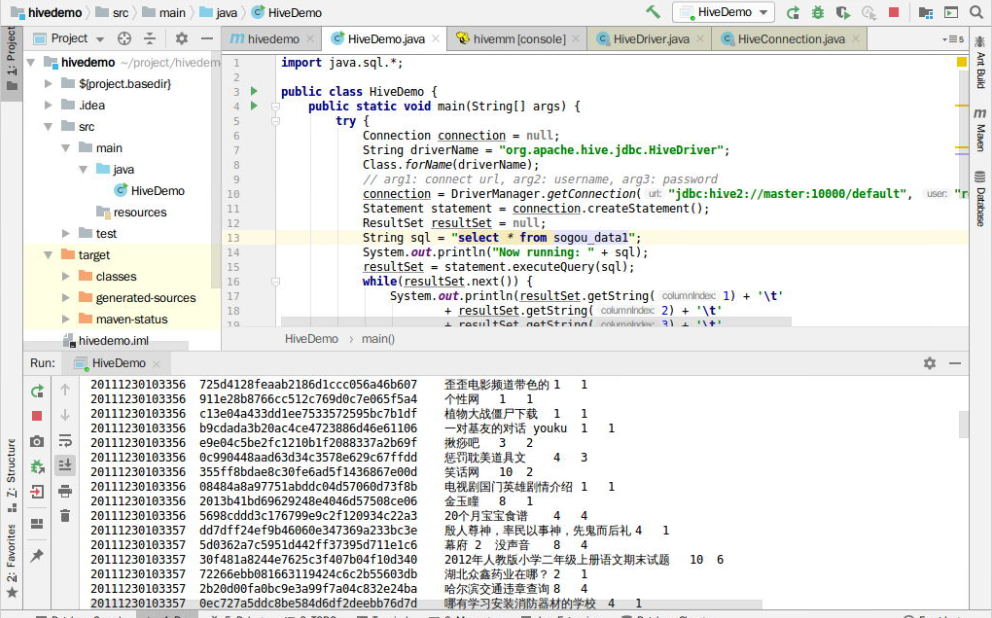
\includegraphics[width=\linewidth]{hive/select.png}
  \caption{Hive JDBC编程运行效果}
  \label{fig:hive-jdbc}
\end{figure}

而且发现,IDEA提供了开箱即用的数据库连接工具,并支持Hive连接。配置成功后即可
在集成开发环境中编写查询语句了,而且提供了很好的语法提示支持,算是一个彩蛋吧。

\begin{figure}[htbp]
  \centering
  \subfloat{
      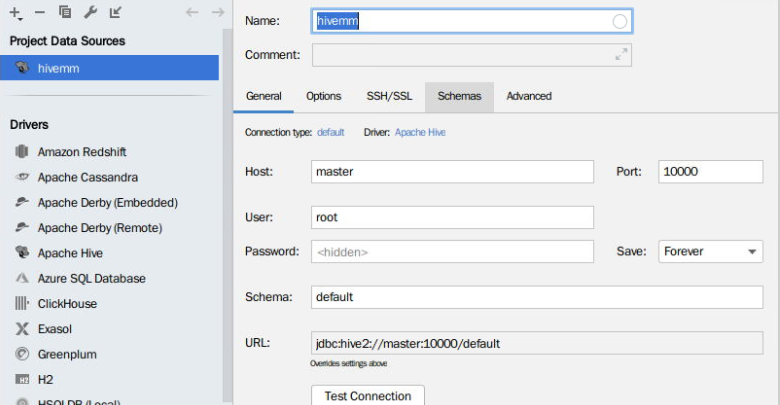
\includegraphics[width=0.48\linewidth]{hive/hiveconfig.png}
  }
  \subfloat{
    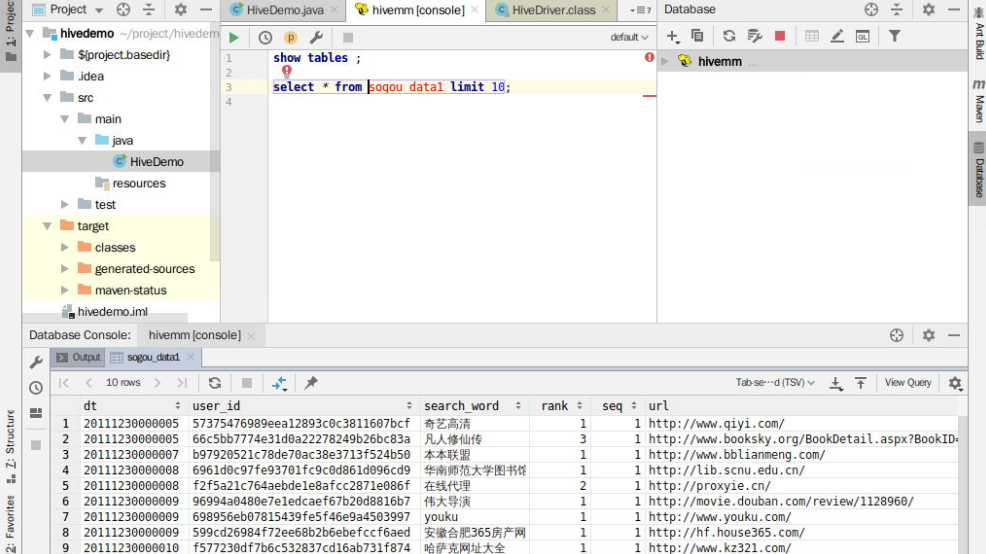
\includegraphics[width=0.48\linewidth]{hive/hivesql.png}
  }
  \caption{IDEA对Hive的良好支持}
\end{figure}
